\section{The chain}
\label{sec:chain}

Figure~\ref{fig:chain} shows how Theorem~\ref{thm:main} rests on its parts.
Table~\ref{tab:chain} lists them in the order of use, with their origin and their units.

\begin{figure*}[t]
\centering
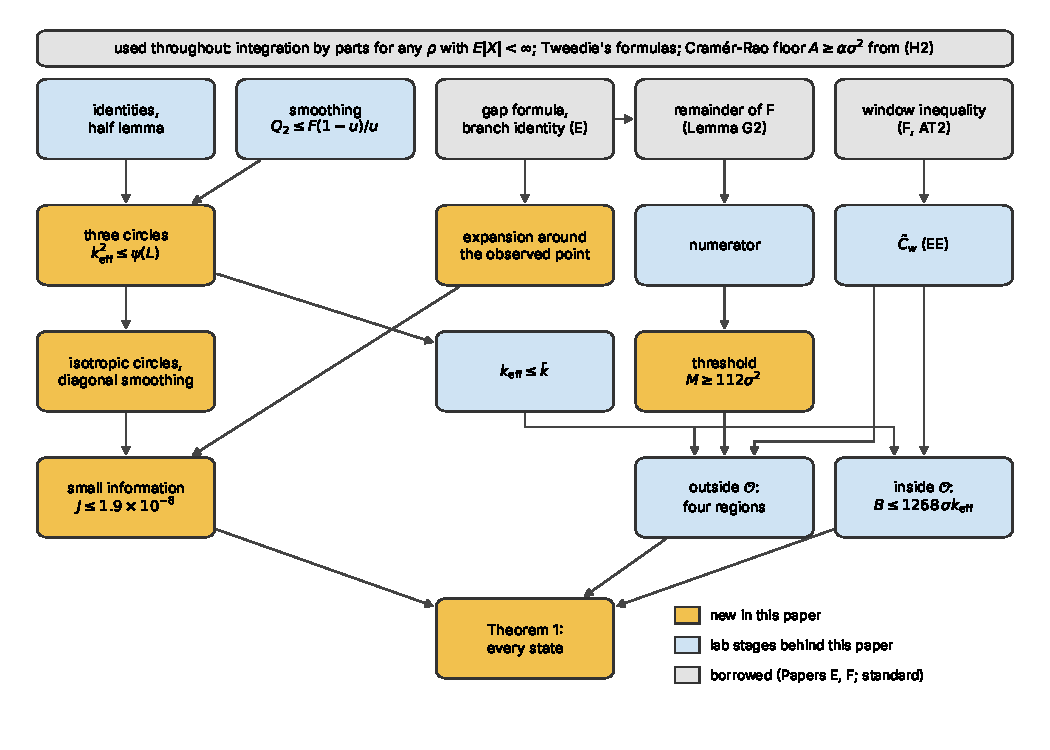
\includegraphics[width=0.8\textwidth]{figures/fig_chain_K.pdf}
\caption{The chain of Theorem~\ref{thm:main}. Boxes are the results of this paper and the borrowed ones (grey); an arrow means ``is used by''. The three new steps are Theorem~\ref{thm:circles} (three circles), Lemma~\ref{lem:EF2} (the threshold that confines every remainder estimate to $\Oset$) and Lemma~\ref{lem:EGD} with Theorem~\ref{thm:EGO} (the expansion around the observed point).}
\label{fig:chain}
\end{figure*}

\begin{table*}[t]
\caption{The parts of the chain in the order of use. Units: ``raw'' are formulas in the original coordinates, ``dimensionless'' are formulas in $\st$, $\Ht$ with $\sigma$ written explicitly, and ``$\sigma=1$'' are formulas for the state $X/\sigma$ with unit noise. Origin: E, F are Papers~E and~F; ED--EH are the lab stages behind this paper; G marks steps proposed by Google Gemini, one of the AI assistants used in this work (see the Acknowledgments).}
\label{tab:chain}
\begin{ruledtabular}
\begin{tabular}{lll}
part & origin & units\\
\hline
Lemma~\ref{lem:ibp} (integration by parts) & EF, EG & raw\\
Lemma~\ref{lem:tweedie} (Tweedie) & standard~\cite{Efron,Robbins} & raw/dimensionless\\
Proposition~\ref{prop:gap} (gap formula) & E, EG & dimensionless\\
Proposition~\ref{prop:branch} (branch identity) & E & dimensionless\\
Lemma~\ref{lem:G2} (remainder of F) & F & raw\\
Lemma~\ref{lem:EF1} (numerator) & EF, G & dimensionless\\
Lemma~\ref{lem:EF2} (threshold) & EF & dimensionless\\
Lemma~\ref{lem:CR} (Cram\'er--Rao floor) & E, EE & dimensionless\\
Lemma~\ref{lem:K} (identities, half lemma) & ED, EF, G & $\sigma=1$\\
Lemma~\ref{lem:smooth} (smoothing) & EF & $\sigma=1$\\
Lemmas~\ref{lem:kernel}--\ref{lem:holo} (circles) & EG, G & $\sigma=1$\\
Theorem~\ref{thm:circles} ($\keff^2\le\psi$) & EG, G & $\sigma=1$\\
Lemma~\ref{lem:window} (window inequality) & F, EE, EF & raw$\to$dimensionless\\
Lemma~\ref{lem:EEC} ($\tilde C_w$) & EE & dimensionless\\
Lemma~\ref{lem:EFO} (inside $\Oset$) & EF & dimensionless\\
Proposition~\ref{prop:outside} (outside $\Oset$) & EF & dimensionless\\
Lemma~\ref{lem:EGD} (direct expansion) & EG & dimensionless\\
Lemmas~\ref{lem:iso},~\ref{lem:sm} (isotropic) & EG, G & $\sigma=1$\\
Theorem~\ref{thm:EGO} (small information) & EG & dimensionless\\
Theorem~\ref{thm:main} & EG, EH, EI & dimensionless
\end{tabular}
\end{ruledtabular}
\end{table*}

Two remarks on the joints.
First, the powers of $\sigma$ change at four places: the Lagrange remainder of Lemma~\ref{lem:G2} (a factor $\sigma^2$), the window inequality (the $\sigma^{-2}$ of $\int(\partial_wf)^2=\keff^2\Jww/\sigma^2$, Lemma~\ref{lem:window}), the bound $B\le\sigma\cdots$ inside $\Oset$ (Lemma~\ref{lem:EFO}), and the remainders $\sigma^2\sqrt J$ and $\sigma\,\Wzz$ of Lemma~\ref{lem:EGD}.
Each of them is checked numerically on recorded states (App.~\ref{app:joints}); the window inequality without its factor $\sigma^2$, which appeared once in the working record, fails there by a factor of $9\times10^{71}$.
Second, the assumptions travel as follows: (M1) enters only through Lemma~\ref{lem:ibp}(ii), used by the gap formula and the branch identity; (H2) enters only through the Cram\'er--Rao floor, $A\ge\alpha\sigma^2$, from which $\ln(1/A)\le\Lb$ and $\keff\le\kb$.
Paper~F's Lemma~BB1 and the ``sufficient decay'' assumed in Papers~E and~F are not used.
